% Created 2024-10-16 śro 21:35
% Intended LaTeX compiler: pdflatex
\documentclass[../../main.tex]{subfiles}

% \usepackage[a4paper, margin=3cm]{geometry}
% \usepackage{amssymb} // not working

\usepackage[T1]{fontenc}
\usepackage[utf8]{inputenc}
\usepackage{graphicx}
\usepackage{longtable}
\usepackage{wrapfig}
\usepackage{rotating}
\usepackage[normalem]{ulem}
\usepackage{amsmath}
\usepackage{capt-of}
\usepackage{hyperref}
\usepackage{siunitx}
\usepackage{float}
\usepackage[polish]{babel}

\graphicspath{{../}}
\author{Wojciech Paderewski}
\date{\today}
\title{Koncepcja ukladu}
\hypersetup{
 pdfauthor={Wojciech Paderewski},
 pdftitle={Koncepcja ukladu},
 pdfkeywords={},
 pdfsubject={},
 pdflang={Polish}}

\begin{document}

Kryterium wyboru buzzera było jego napięcie zasilania, głośność oraz jak najmniejszy rozmiar.
Wybrano buzzer CEM120342, jest to buzzer piezoelektryczny. Z noty katalogowej \cite{st:buzzer} wypisano użyteczne parametry na etapie projektowania:

\begin{itemize}
    \item Napięcie zasilania: 3-5 V
    \item Max prąd zasilania: 35 mA
    \item Częstotliwość: 2,048 kHz
    \item Głośność: 85dB - 95 dB
    \item Średnica: 12mm, wysokość: 8 mm
    \item Rezystancja: \SI{42}{\ohm}
    \item Typ montażu: THT
\end{itemize}

Buzzer został podłączony według schematu zalecanego przez producenta przedstawionego na rysunku \ref{fig:buzzer_karta}.
\begin{figure}[H]
    \centering
    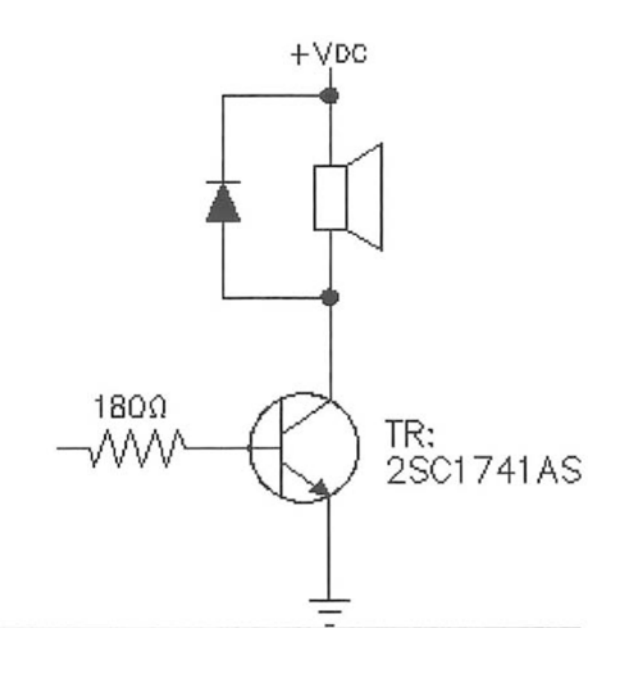
\includegraphics[width=0.65\textwidth]{buzzer_karta.png}
    \caption{Schemat zalecany przez producenta \cite{st:buzzer}}
    \label{fig:buzzer_karta}
\end{figure}

Do sterowania wykorzystano inny tranzystor,
użyto tranzystora który służy do sterowania katodami kropek w lampach nixie, by nie dodawać kolejnego elementu do projektu.
Tranzystor ten ma prąd kolektora 80 mA, co jest wystarczające do sterowania buzzerem.
Buzzer jest dostatecznie mały, jedyną wadą jest montaż THT, który ogranicza miniaturyzację płytki drukowanej.
Schemat elektryczny złącza z buzzerem przedstawiono na rysunku \ref{fig:buzzer}.


\begin{figure}[H]
    \centering
    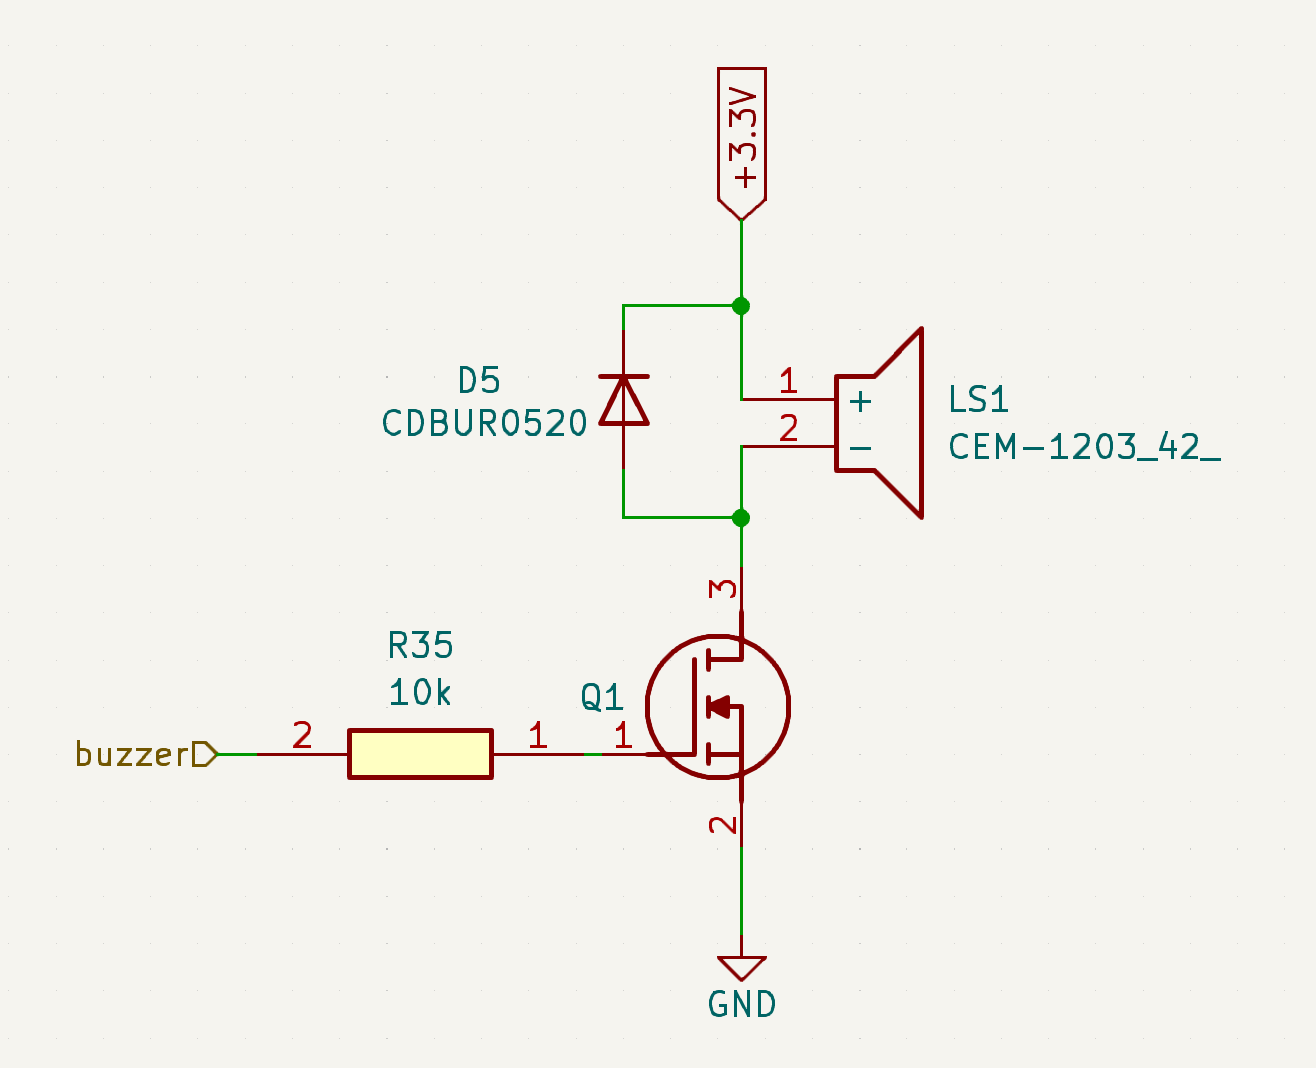
\includegraphics[width=0.8\textwidth]{buzzer.png}
    \caption{Schemat elektryczny podłączenia buzzera}
    \label{fig:buzzer}
\end{figure}

\end{document}
